\section{Data}

\subsection{Light Bulbs and the Solar spectrum}
For this part, we found the index of the peak, and used the corresponding
wavelength in \cref{eq:wien} to calculate the temperature $T$.

\begin{equation}
    T_{\text{H}} = \SI{4736}{\kelvin}, \quad T_{\text{D}} =
    \SI{4842}{\kelvin}, \quad T_{\text{E}} = \SI{4829}{\kelvin}
\end{equation}

\begin{figure}[h!]
\centering
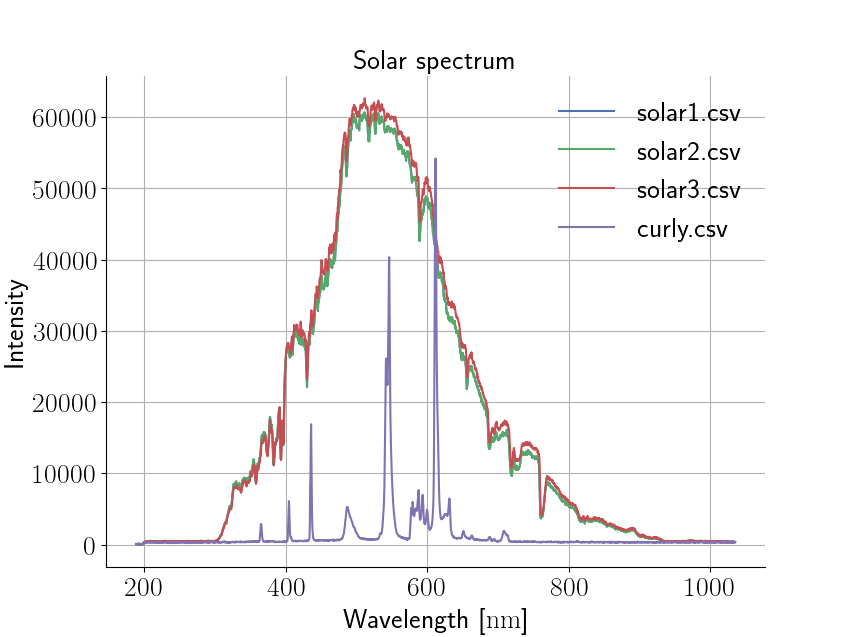
\includegraphics[width=0.65\textwidth]{SolarComparison0}
\caption{The spectrum of the diode-based lamp compared to the three meassured spectra of
the sun.} 
\label{diode}
\end{figure}

\begin{figure}[h!]
\centering
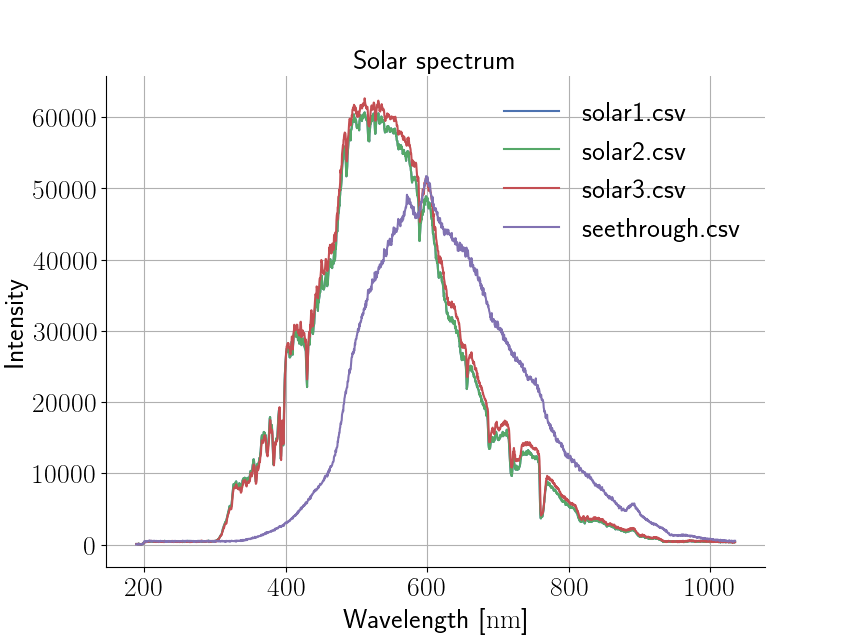
\includegraphics[width=0.65\textwidth]{SolarComparison1}
\caption{Halogen}
\label{halogen}
\end{figure}

\begin{figure}[h!]
\centering
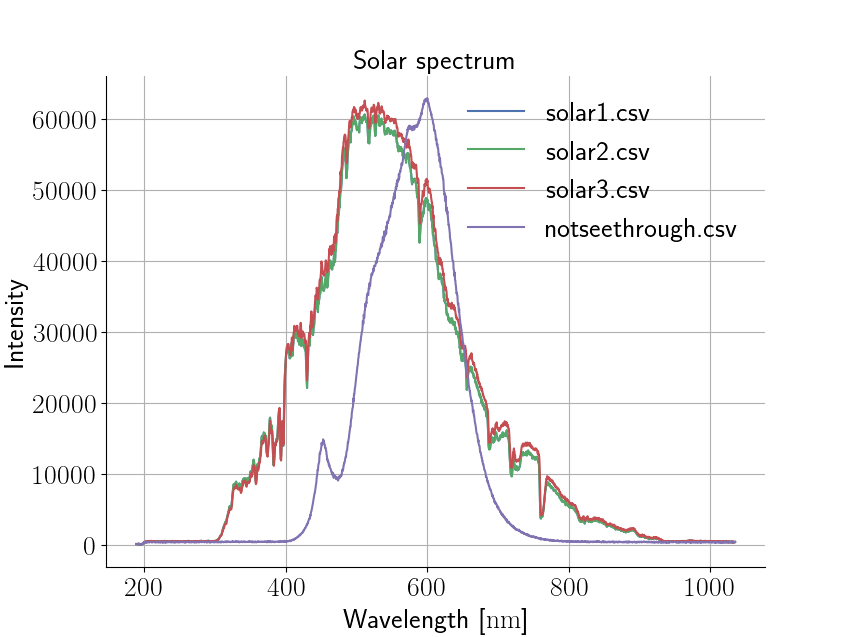
\includegraphics[width=0.65\textwidth]{SolarComparison2}
\caption{Energy-saving lamp}
\label{Energy-saving}
\end{figure}

\subsubsection{Comparison}
\fxnote{HERE}

\subsection{Fraunhofer lines}
\begin{figure}[h]
\centering
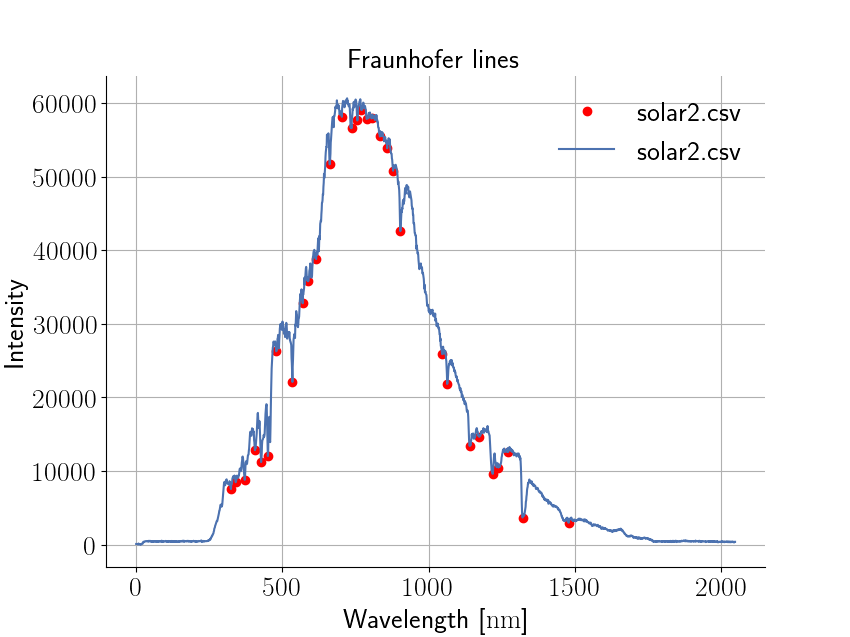
\includegraphics[width=0.5\textwidth]{Fraunhofer}
\caption{The Solar spectra with the local extrema points used for
classification of the Fraunhofer lines}
\label{frauenhofer}
\end{figure}

Comparing the found extremas with the Fraunhofer lines, we have meassured the
following

